% Event omission reasons for supplementary material

\paragraph{Event omissions.} The full list of reasons for omission
is given below, with the descriptive code for the reason in bold
typeface and the number of occurrences (out of 17617 events) in
italics.

% Never occurs
% \paragraph{ 1 target posn change insignificant}
% masked by reason 3

% Never occurs
% \paragraph{ 2 target posn held less than min. duration}
% This is Mauro's event duration, which I couldn't understand and so I
% turned this feature off.

% Code 3. 410 occurrences (these mask omit reason 1)
\paragraph{\emph{Target position change less than minimum jump size:}} If the
target line's position changed less than a threshold of 20 pixels, it
was omitted from analysis. This was used to allow the output of the
script to be compared with an alternative method for measuring latency
and error rates, described later. \emph{410 occurrences.}

% 120 occurrences for Async distractors
\paragraph{\emph{Stable position later than event onset:}} If the stylus did not
achieve a stable pre-event position, then it was not safe to measure a
latency for the movement for the event. This usually occurred when two
target events followed each other in quick succession and the subject
had not had time to reach the first target position before it moved
for a second time. \emph{120 occurrences.}

% Never occurs
%\paragraph{ 5 Another event caused this movement}
%
%When two distractors occur close in time together, any movement of the
%stylus should be ascribed to one event only. In the later of two
%distractor events, this is set as the omit reason.

% Never occurs
%\paragraph{ 6 Not distracted}
%
%If a movement is detected following a distractor event, but it is a
%movement \emph{away} from the distractor, then this is given as the
%omit reason. Usually, the movement will be towards a subsequent target
%event.

% Codes 7 and 8. 130 occurrences (targ) 20 occurrences (distractor)
\paragraph{\emph{Too fast (targ)}} and {\bf \emph{Too fast (distractor):}}
% 100 ms is the value of A.fastest\_brain\_decision
Any event with a movement latency below 100~ms (the value of the
parameter \codeparam{A.fastest\_brain\_decision} in the
\filename{lt\_analyse\_latency.m} script) was omitted. Previous research
suggests that participants cannot make movements faster than this
\cite{gielen_coordination_1984,prablanc_optimal_1979}. The cause of
such apparently short latencies in the raw data was usually the lack of
a stable pre-event stylus position; the subject was not able to settle
at the previous target position. \emph{130 occurrences (target), 20
  occurrences (distractor).}

% Code 9. 21 occurrences
\paragraph{\emph{No movement detected}}

No movement was detected for a target event, and therefore no latency
could be determined. This may have occurred if the target position
change was very small. \emph{21 occurrences.}
% Find example

% Code 10. No occurrences
%\paragraph{ Failed to find stable stylus posn}
% Occurs if cur events pos_move_thresh > max_move_thresh. This may
% occur if the stable position was very wobbly

% Code 11 731 occurrences for targets, 1743 occurrences for distractors
\paragraph{\emph{Stable stylus period too short}}

If the stable stylus position period was less than 200~ms for targets
(\codeparam{A.min\_stableposition\_period}) or 150~ms for distractors
(\codeparam{A.min\_stableposition\_period\_dist}) then the event was
omitted, which is to say that a latency was measured only if the
stylus remained in a stable position for at least the above periods of
time. It was the second most common reason for omitting an event from
latency and error measurements. \emph{731 occurrences (target), 1743
  occurrences (distractor).}

% ADD FIGURE HERE to illustrate

%  lack of a stable pre-event stylus position:
%  E.g. Katie/GM/line/20141201142107 (Ev 47 I think) or
%  Olivia/RG/line/20141204142043 (Ev 37)

% Code 12. 21 occurrences for targets, 18 for distractors
\paragraph{\emph{Drift too great during stable stylus period}}
If the stylus position at the end of the stable stylus period had
moved more than 15 px (\codeparam{A.max\_move\_thresh}) with respect
to the stylus position at the start of the stable stylus position
period, then the event was omitted with this reason.  \emph{21
  occurrences (target), 18 occurrences (distractor).}

% Code 13. 1820 occurrences for targets, 957 for distractors
\paragraph{\emph{Drift too great during stable period (avg)}} If
the average speed of the stylus during the stable stylus period was
greater than a threshold of 0.01~px/ms (0.011~cm/s) for a target event
(\codeparam{A.max\_avg\_drift\_speed}) or 0.02 px/ms (0.023~cm/s) for
a target event (\codeparam{A.max\_avg\_drift\_speed\_dist}) then the
event was omitted. Because the mean time between target events was set
to 1.2 s, a fast rate, this was the most common reason for omitting
movements from analysis. \emph{1820 occurrences (target), 957
  occurrences (distractor).}

% A nice example of drift is too great is in
% Rachel/HY/line/20141118151002.txt (ND) event 8.
\begin{figure}[htb!]
\centering
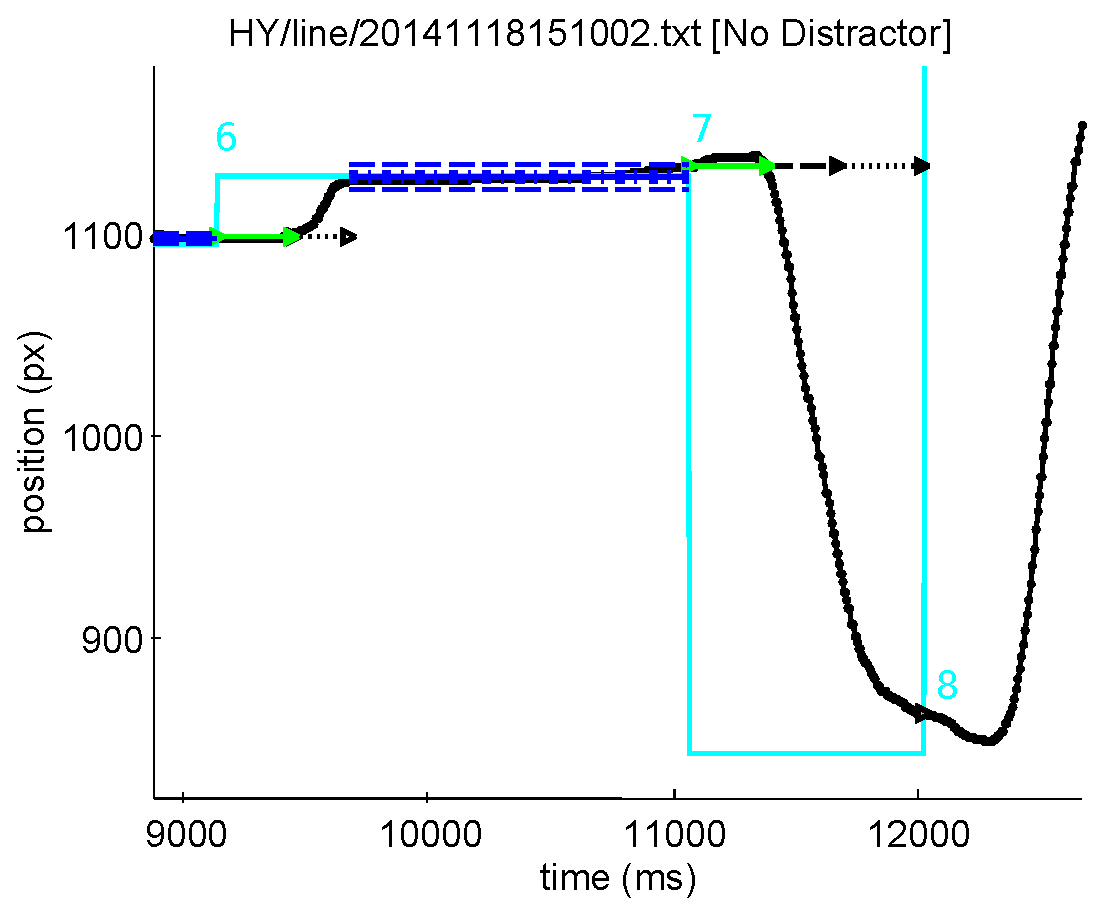
\includegraphics[width=0.5\textwidth]{./figures/drift_too_great_nolegend.eps}
\caption[Drift too great] {An example event for which the omission
  reason was ``Drift too great during stable period (avg)''. Here, the
  latency onset for events 6 and 7 were determined, but the stylus
  (black line) did not become stationary at the target position (cyan
  line) prior to event number 8 and so it was omitted from latency and
  error analysis. For the meaning of line colours, refer to
  Fig.~\ref{example_event}.}
\label{omission_reason_8}
\end{figure}


% Code 14. No occurrences. Masked by ``drift too great''.
%\paragraph{Stylus moving at event onset}

% Code 15. No occurrences
%\paragraph{Stylus didn't move away from target}
% This is coded to occur if the distracted motion occurs beyond the
% \emph{next} distractor event. Presumably masked by alternative
% reasons for no motion detected.

% Code 16. 1756 occurrences
\paragraph{\emph{Movement occurs beyond next target}}
This omit reason was recorded for a distractor event when any detected
motion occurred after the next target event. It means that the subject
did not make an error movement, and therefore no latency could be
measured. However, these distractor events \emph{were} included when
computing the proportion of distractor events which caused an error
movement. \emph{1756 occurrences (distractor).}

% 4 occurrences. distractor event leads target event. Same dirn
\paragraph{\emph{Subject was distracted by closely previous distractor}}
These last four reasons for omission concern the case where there was
an asynchronous distractor and a distractor event and target event
occur temporally close together. In this particular case, either the
target or the distractor may have caused the movement; both lines were
displaced in the same direction with respect to the stable stylus
position. The distractor event occurred before the target
event. Because the recorded motion was \emph{away} from the target,
the target was omitted and the event was recorded as a distraction in
the earlier distractor event.  \emph{4 occurrences (target).}

% 7 occurrences. distractor event leads target event. Diff dirns
\paragraph{\emph{Incorrect move was recorded in previous distractor event}}
In this case, the target and distractor lines were located in opposite
directions from the initial stylus position; again, the distractor
line occurred first. The stylus initially followed the distractor and so
an incorrect movement was recorded in the distractor event, and the
target event was omitted with this reason code. \emph{4 occurrences
  (target).}


% 66 occurrences. target event leads distractor event.
\paragraph{\emph{This distractor event did not distract the stylus movement}}
In this case, the target event led the distractor event and they
had opposite directions. The stylus successfully followed the target
event and so the distractor event, which occurred soon after was omitted
with this reason.  \emph{66 occurrences (distractor).}

% 4 occurrences for distractor. target event leads distractor event.
\paragraph{\emph{Recorded this stylus movement as a distraction towards the next distractor}}
Again, the target event led the distractor event and they had
opposite directions. Here, the stylus followed the distractor direction
and so to avoid recording a second movement error, the target event was
omitted. \emph{4 occurrences (target).}
